\section{Grain growth/shrinkage of a spherical grain}
\label{sec:example_graingrowth}
\subsection{Preliminaries}
\label{sec:example_graingrowth_prelim}
A spherical grain will shrink due to its curved interface in order to minimize the interface energy. Doing so, the grain retains its sperical shape 
while the radius decreases with time.\\

From theoretical considerations, an analytic formalism can be can be found which describes the kinetics of this shrinkage. This example simulation should reproduce this dependence.
Starting with the phase-field equation for two phases
\begin{equation}
\dot\phi = \mu \left(\sigma \left(\nabla^2\phi+ \frac{\pi^2}{2\eta^2}(2\phi-1)\right) + \Delta G\right)
\label{eq:graingrowth_singlegrainpde}
\end{equation}
with $\sigma$ being the interfacial energy, $\mu$ the mobility parameter and $\Delta G$ any additional driving force, 
For the grain boundary evolution when particle radius $R \ll \eta$, an approximate 
theoretical time dependence of the grain radius can be obtained ($\Delta G = \si{0}{J/m^3}$). At time $t=0$ the sphere radius is $R_0$. In the interface of width $\eta$, the phase-field is expressed in spherical coordinates
\begin{equation}
    \phi(r)= \frac{1}{2} - \frac{1}{2}\sin\frac{\pi(r-R)}{\eta}
\end{equation}
and noting that 
\begin{equation}
    v=-\frac{dr}{dt}=\dot\phi\frac{\partial r}{\partial \phi}
\end{equation}
one can obtain the following growth relation
\begin{equation}
    R^2-R_0^2=-4\sigma t.
\end{equation}

\subsection{Modules and parameters}
\label{sec:example_graingrowth_setup}
The benchmark uses the three mandatory modules \nameref{sec:module_phasefield}, \nameref{sec:module_boundaryconditions} and \nameref{sec:module_settings}. Moreover, the modules \nameref{sec:module_interfacefield}, \nameref{sec:module_interfaceenergy} and \nameref{sec:module_interfacemobility} are required. A spherical grain of phase 1, initial radius $R_0$, surrounded by phase 0 is considered. The grain is
placed in the center of a cubic box with zero-gradient boundary conditions. No
driving force is applied.\\

The box size is 64x64x64 grid points. The input parameters are listed in table~\ref{tab:graingrowth_setup}.
%\sisetup{scientific-notation = scientific}
\begin{table}
\centering
\begin{tabularx}{0.5\textwidth}{lr} 
\toprule
Parameter & Value\\ 
\midrule 
$N_x=N_y=N_z$ & 65\\
$\Delta x$ & \SI{1e-6}{m}\\
$\eta$ & $5\cdot \Delta x$\\
$\mu$ & \SI{4e-9}{m^4/(J s^2)}\\
$\sigma$ & \SI{0.24}{J/m^2}\\
$\Delta t$ &  \SI{1e-5}{s}\\
$R_0$ & $N_x/3$\\
\bottomrule
\end{tabularx}
\caption{Setup parameters}
\label{tab:graingrowth_setup}
\end{table}

\subsection{Results}
\label{sec:example_graingrowth_results}
The output data in .vts format is written in the VTK directory and can be directly 
visualized using Paraview software (www.paraview.org). The R\_2\_graph.dat file contains the values of the time step and the particle radius calculated analytically and numerically.
Figure~\ref{fig:graingrowth_singlegrainsim1} shows the results of $R^2$ over timesteps for different values of $\eta$. Obviously, a wider interface width improves result towards the analytic solution, yet at the price of higher calculation costs. In addition, simulation with constant driving forces $\Delta G_{\alpha\beta}$ (Matrix $\alpha$, Phase $\beta$) are performed and compared against the solution shown above. Here, however, the solution for equation (\ref{eq:graingrowth_singlegrainpde}) can only be obtained numerically. Figure \ref{fig:graingrowth_singlegrainsim2} compares the solution of OpenPhase with these solutions.
\begin{figure}[p]
\centering
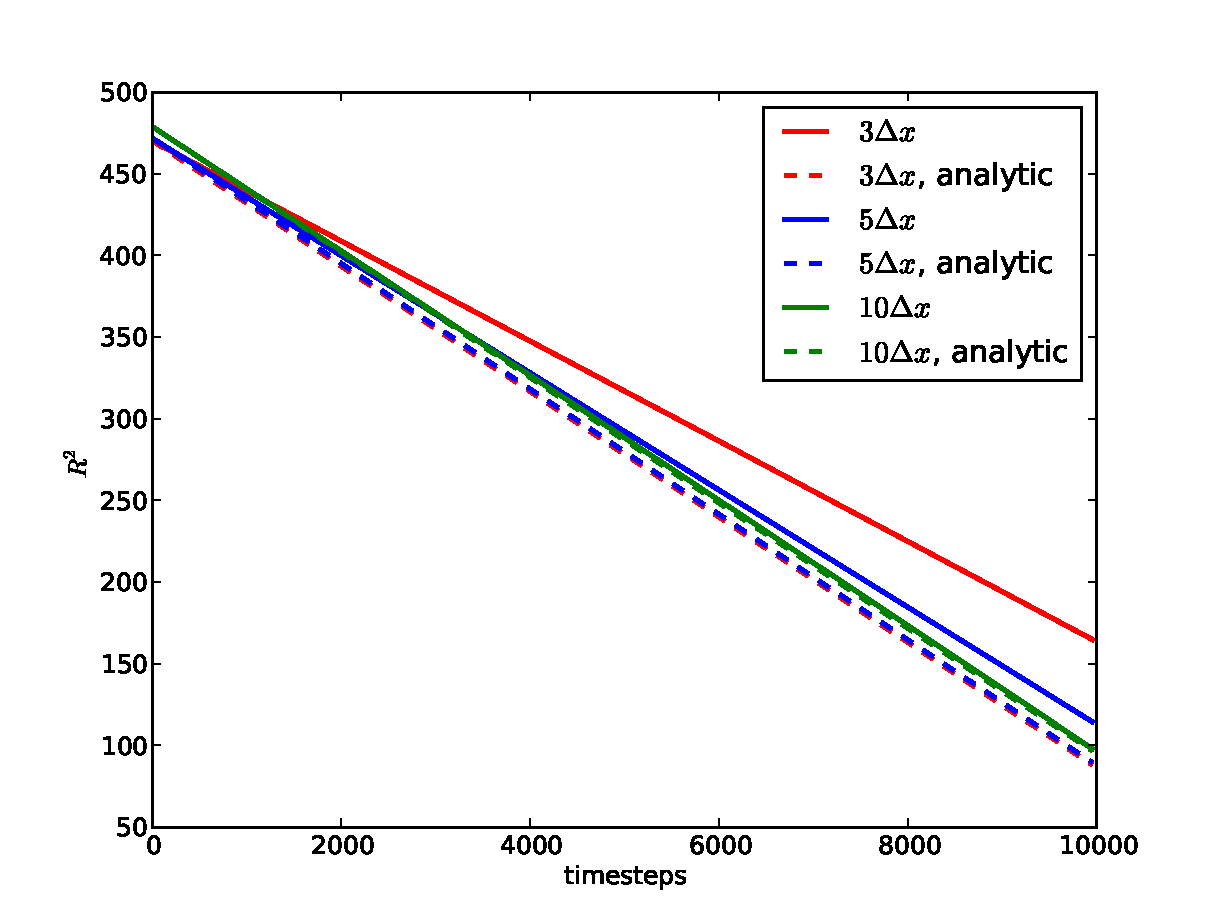
\includegraphics[width=0.8\textwidth]{Figures/examples/R2NDIF.pdf}
\label{fig:graingrowth_singlegrainsim1}
\caption{$R^2$ of sphere radius for different interfacial widths. Comparison with analytical solution (dashed lines).} 
\end{figure}
\begin{figure}[p]
\centering
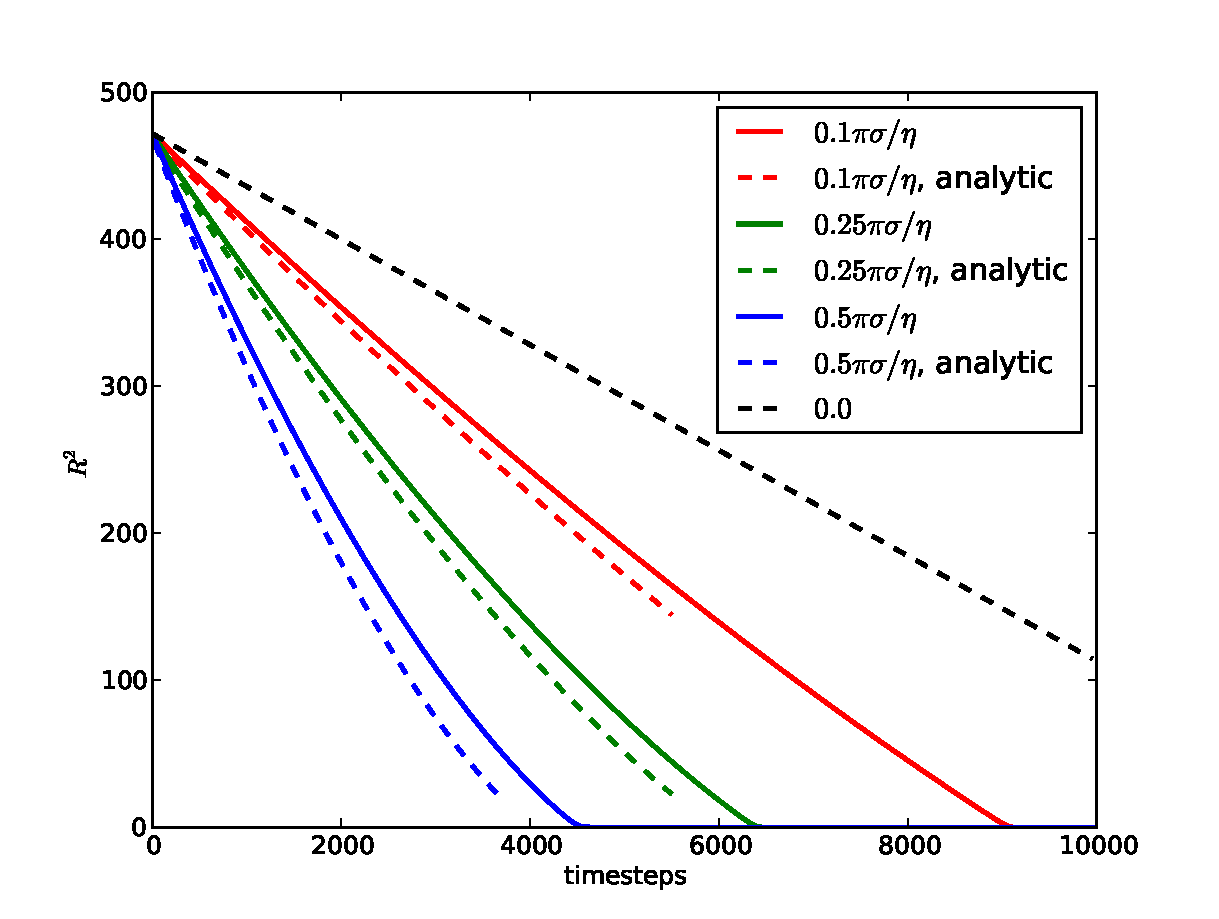
\includegraphics[width=0.8\textwidth]{Figures/examples/R2DDF.pdf}
\caption{$R^2$ of sphere radius for different constant driving forces $\Delta G_{\alpha\beta}$. Comparison with analytical solution (dashed lines).}
\label{fig:graingrowth_singlegrainsim2}
\end{figure}

As a further example, the influence of a elastic driving forces should be benchmarked. Therefore, an eigenstrain of $\varepsilon_{11}=\varepsilon_{22}=\varepsilon_{33} = 0.005$ is defined for the inclusion. The elastic constants for inclusion and matrix are taken equally (see Eshelby example). Free stress boundary conditions are applied, $\bar\sigmaB = 0.$ The results are shown in figure~\ref{fig:graingrowth_singlegrainsim3}. Obviously, the driving force remains constant throughout the shrinkage of the grain. Looking at the analytic solution of the stress field as derived by Eshelby, eq.~(\ref{eq:EshelbyTest_AnalyticalSolution}), the maximum stress in the interface does not depend on the inclusion diameter, but only on the eigenstrain magnitude. Consequently, the elastic driving force (\ref{eq:module_elasticityreuss_drivingforce}) has to remain constant, as reflected by the analytical solution.
\begin{figure}
\centering
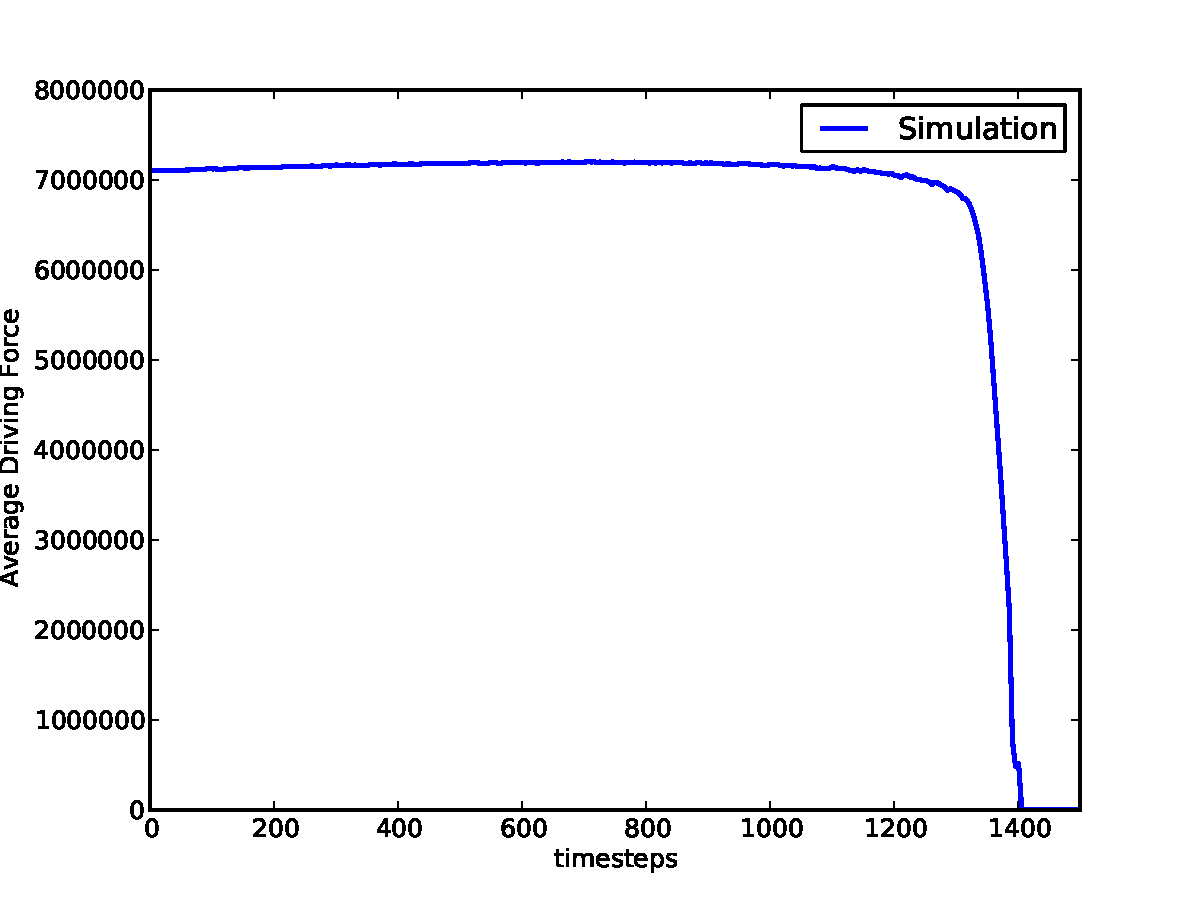
\includegraphics[width=0.8\textwidth]{Figures/examples/AveragedDF.pdf}
\caption{Average driving force in the interface during shrinkage of grain.}
\label{fig:graingrowth_singlegrainsim3}
\end{figure}
